\documentclass[a4paper,10pt,twocolumn]{memoir}
\usepackage[utf8]{inputenc}
\usepackage[T1]{fontenc}
\usepackage{lmodern}
\usepackage{xcolor}
\usepackage{tikz}
\usepackage{geometry}
\usepackage{graphicx}
\usepackage{amsmath,amssymb}
\usepackage{hyperref}
\usepackage{tocloft}
\usepackage{parskip}
\usepackage{enumitem}
\usepackage{microtype}
\usepackage{fancyhdr}
\usepackage{lettrine}
\usepackage{tikz}
\usetikzlibrary{shapes.geometric, arrows, positioning}


% Page geometry
\geometry{
  a4paper,
  left=15mm,
  right=15mm,
  top=20mm,
  bottom=15mm,  % Reduced bottom margin
  columnsep=8mm
}

% Color palette
\definecolor{primary}{RGB}{30, 50, 100}
\definecolor{accent}{RGB}{200, 80, 0}
\definecolor{light}{RGB}{245, 245, 248}
\definecolor{dark}{RGB}{40, 40, 45}
\definecolor{gray}{RGB}{120,120,120}  % Defined gray color

% Typography
\renewcommand{\familydefault}{\sfdefault}
\setlength{\parindent}{0pt}
\setlength{\parskip}{0.7em}  % Slightly tighter paragraph spacing
\linespread{1.05}
\frenchspacing

% Header/Footer
\pagestyle{fancy}
\fancyhf{}
\fancyhead[L]{\footnotesize\scshape\color{primary}The Aevum}
\fancyhead[R]{\footnotesize\color{primary}June 2025}
\fancyfoot[C]{\thepage}
\renewcommand{\headrulewidth}{0.4pt}
\renewcommand{\headrule}{\hbox to\headwidth{\color{accent}\leaders\hrule height \headrulewidth\hfill}}

% Article command
\newcommand{\article}[3]{
  \section*{#1}
  \addcontentsline{toc}{section}{#1}
  \begin{center}
    \color{dark}\normalsize\textbf{#2}\\
    \small\color{gray}#3
  \end{center}
  \vspace{-0.8em}  % Tighter spacing
}

% Compact Contributors command
% Modified contributor command without image, but with roll and registration numbers
\newcommand{\contributor}[4]{%
  \vspace{0.4em}
  \begin{minipage}{\textwidth}
    \textbf{\normalsize #1}\\
    {\footnotesize Roll: #2 \quad Reg: #3}\\
    {\footnotesize\color{gray}#4}
  \end{minipage}
}


\begin{document}

% Front Cover
\begin{titlingpage}
\thispagestyle{empty}
\begin{center}
\vspace*{1.5cm}
{\fontsize{42}{50}\selectfont\bfseries\color{primary}The Aevum}
\vspace{0.5cm}

{\Large\scshape\color{accent}YESTERDAY-TODAY-ALWAYS}
\vspace{1.5cm}

\tikz{\draw[accent, line width=1pt] (0,0) -- (8cm,0);}
\vspace{1cm}

{\Huge\bfseries\color{dark}JUNE 2025}
\vspace{0.2cm}

{\large Volume 1 • Issue 1}
\vfill

{\large\bfseries Featured Articles}\\[0.5em]
{\color{dark}
The Silent Revolution\\
Ghostwriting in Technical Writing: An Ethical Dilemma \\
Cloud Security: Guarding Your Digital Vault\\
Machine-Learned Muscles: Personalized Performance through AI\\
Quantum Computing: Unlocking the Future of Computation\\
Quickstart in Robotics and Microcontrollers: A Beginner's Journey\\
Dopamine: The Currency of Digital Control}
\vfill

{\small\scshape\color{gray}Produced by NeuroNumb}
\end{center}
\end{titlingpage}

% Table of Contents
\clearpage
\tableofcontents*
\thispagestyle{empty}
\clearpage
\cleardoublepage
\newpage

% ====================
% START OF ARTICLES
% ====================

% Article 1
\article{\centering{The Silent Revolution}}{Muhaimin Kamran}{June 17, 2025}
\lettrine[lines=3]{O}{nce} \textbf{science fictions} were dismissed as mere fantasy. In 1864, \textbf{Jules Verne} wrote \textit{Journey to the Center of the Earth}, where he described a mission to the Moon—launched from Florida. Then, in 1870, he penned \textit{20,000 Leagues Under the Sea}, in which \textbf{Captain Nemo} traveled beneath the ocean in an electric-powered submarine. Decades later, in 1969, \textbf{Neil Armstrong} stepped onto the Moon during the Apollo 11 mission—and science fiction began turning into reality. Today, detailed underwater exploration is routine. \textbf{Sci-fi started becoming real}.

In January 2024, the first successful \textbf{brain-computer interface (BCI)} was implanted—a tiny device in the brain allowing humans to interact directly with computers, AI, or prosthetics. \textbf{Noland Arbaugh}, a young man left quadriplegic after a diving accident, became the first human subject. \textbf{Neuralink} implanted a chip—called the \textbf{“Link”}—into the region of his brain that controls movement. The chip has sixty-four threads, each thinner than human hair, placed precisely by a \textbf{surgical robot}. With it, Noland can move a computer mouse using only his thoughts. He now browses the internet, plays chess, and navigates online tools without moving a single muscle. Neuralink even livestreamed him playing chess on a MacBook using only brain signals. By mid-June 2025, \textbf{BCI’s initial implementation had proven successful}. \textbf{dshufliaf}. 

Meanwhile, AI systems, especially those developed by \textbf{OpenAI} and others—have performed remarkably well in standardized exams designed for humans. For example, AI passed all three steps of the \textbf{USMLE} (medical licensing exam), scored in the \textbf{top 10\%} on the \textbf{Bar Exam}, and placed around the 90th percentile on the \textbf{LSAT} (law school admission test). It scored between 1400 and 1550 on the \textbf{SAT} and performed at around the 99th percentile in verbal reasoning and 85th percentile in quantitative reasoning on the \textbf{GRE}. On \textbf{AP exams}, AI typically scores \textbf{4s and 5s}. On top of that, it solves coding challenges across platforms like \textbf{LeetCode} and in competitive programming environments.

AI has also discovered \textbf{Halicin}—a novel antibiotic—by exploring chemical spaces that no human ever had. \textbf{DeepMind’s AlphaFold} predicted the 3D structure of nearly every known protein. AI can now generate full software apps, websites, scripts, even games—just from a prompt. AI tools produce short films, stunning artwork, and realistic human faces that don’t exist. \textbf{DeepMind’s AlphaStar} has beaten \textbf{99.8\%} of all human \textit{StarCraft II} players.

We once dreamed of the future. \textbf{Now, the future has awakened—before we were ready}.

In the coming years, we may see \textbf{mass adoption of BCIs}. Human thinking, analysis, and imagination could begin to merge with real-time internet data. It may even become possible for someone to \textbf{spy on our thoughts}.

\textbf{AI-powered robo-doctors} or \textbf{AI judges} may become mainstream—cost-effective, efficient, and widely accessible. At the same time, AI capable of exploring chemical spaces might design \textbf{deadly pathogens}. Automated law enforcement systems could operate with no empathy or human oversight. Governments may use legal AI to justify censorship or oppression. Fake videos, false news, and synthetic war footage will become harder to detect. Identities may be lost, as AI perfectly mimics faces, voices, and writing styles.

\textbf{These technologies are advancing faster than the laws that govern them.} If left unchecked, tools designed to empower humanity could destabilize it. Regulation does not mean halting progress, it means steering it toward safe, fair outcomes.

\textbf{We are not yet at the point where AI thinks independently, like in science fiction.} But we are moving faster than we ever imagined. The convergence of AI, brain interfaces, and quantum computing marks a profound turning point in human history.

These tools carry tremendous promise—cures for diseases, universal access to knowledge, freedom from disability, and global efficiency. But without thoughtful regulation, rigorous testing, and transparent governance, they may also introduce risks for which we are not yet prepared. \textbf{We do not fear the future; we fear that it is already here}.
\clearpage
\cleardoublepage

% Article 2
\article{\centering{Ghostwriting in Technical Writing: An Ethical Dilemma }}{Maliha Laheen}{June 17, 2025}
\lettrine[lines=3]{T}{echnical}
% Introducing the concept of ghostwriting
 writing involves creating documents like instruction manuals, reports, and guides used in fields such as technology, medicine, or engineering. These documents must be clear and accurate. However, sometimes the person who writes them does not receive credit. This practice, known as ghostwriting, occurs when someone writes a document, but another person’s name, such as a boss or a company, appears as the author. While common, it raises questions about fairness and transparency. Should readers know who wrote the document? This article explores why ghostwriting matters and whether openness could make these documents more trustworthy.

% Exploring the ethical implications
\section*{The Ethical Core: Is Ghostwriting Dishonest?}
Ghostwriting can feel misleading. If the person listed as the author did not write the document and lacks deep knowledge of the subject, problems may arise. For instance, a poorly written guide for a medical device could cause harm if it contains errors. On the other hand, ghostwriting can be practical. Companies hire skilled writers to ensure documents are clear and correct, even if the company itself is not an expert.

This creates a balance between honesty and efficiency. Some argue readers should know the writer’s identity to judge the document’s reliability. Others believe the accuracy of the information is more important than who wrote it.

% Reflecting on the philosophical aspects of authorship
\section*{Philosophical Reflections: Who Should Get Credit?}
Typically, the person who writes something is considered the author and is responsible for its content. Ghostwriting changes this dynamic. The writer remains hidden, while someone else takes credit—and responsibility if issues occur. For example, if a manual is unclear and leads to a mistake, who is at fault: the writer or the person named as the author?

One perspective supports ghostwriting if it results in better documents that benefit users. However, another view considers it unfair to conceal the true writer. This raises a question: Does being an author mean doing the work, receiving recognition, or both?

% Discussing the challenges faced by ghostwriters
\section*{The Ghostwriter’s Challenge: Working Without Credit}
Ghostwriters face a difficult task. They must write accurately and clearly while aligning with the client’s preferences, all without public recognition. This lack of credit can feel unfair—why should someone else be praised for their work?

Ghostwriters also strive to maintain accuracy, sometimes disagreeing with clients to ensure correctness. Since their names are not attached, it can be hard to feel fully accountable. Revealing the writer’s role might help, but it could complicate matters or make the client appear less knowledgeable.

% Presenting a case study to illustrate risks
\section*{Case Study: When Ghostwriting Causes Problems}
Consider a scenario where a ghostwriter creates a report about a new medical device, credited to a well-known doctor. If the report contains mistakes and the device fails, people may blame the doctor, who did not write it. This confusion can reduce trust in the report. Had the ghostwriter’s involvement been disclosed, readers might have reviewed it more carefully, potentially avoiding the issue. This example highlights the risks of hiding the true writer.

% Proposing guidelines for ethical ghostwriting
\section*{Guidelines for Ethical Ghostwriting}
To make ghostwriting fairer, consider these suggestions:
\begin{enumerate}
    \item \textbf{Be Honest}: Whenever possible, indicate who wrote the document, even subtly.
    \item \textbf{Own the Work}: The credited author should review the document and ensure its accuracy.
    \item \textbf{Focus on Truth}: Writers should prioritize factual correctness, even if clients suggest otherwise.
    \item \textbf{Give Some Credit}: Acknowledge the writer’s contribution, even privately.
\end{enumerate}
These steps could improve ghostwriting practices for everyone involved.

% Concluding with a balanced perspective
\section*{Conclusion: Finding the Right Way}
Ghostwriting is valuable for producing clear documents but raises concerns about fairness and responsibility. Transparency about authorship might be the most honest approach, though it is not always practical. By considering both the benefits and challenges, ghostwriting can be used thoughtfully. The goal is to ensure these documents are reliable and helpful for those who depend on them.
\clearpage 
\cleardoublepage
% PASTE ARTICLE 2 CONTENT HERE

% Article 3
\articlev{Cloud Security: Guarding Your Digital Vault}}{Ferdous Ara Fahima}{June 17, 2025}
\lettrine[lines=3]{W}{hat} 
 if your bank account was suddenly drained because someone cracked your online banking app? Or your private emails were splashed across the internet? That’s the kind of chaos a cloud breach can unleash. Cloud computing—your email, your company’s CRM, even your favorite photo app—runs our world, but it’s also a hacker’s playground. Why do they keep getting in, and what’s stopping them? Cloud security is our defense line, a mix of clever tech and sharp strategy to keep our data locked tight. Let’s crack open the vault and see how we can keep the bad guys out in 2025 \cite{csrc2024}.

\section*{The Pillars of Cloud Security}

Building a secure cloud is like designing a bank vault: you need strong locks, tight access, and constant vigilance. Let’s meet the core pieces holding it together.

Encryption is your data’s bulletproof vest. It turns your files into a secret code only the right key can unlock, whether they’re stored or moving online. Think AES-256, the kind of lock even supercomputers struggle with \cite{cloudsec2025}. Identity and Access Management (IAM) is your vault’s security guard, checking credentials before letting anyone in. Multi-factor authentication (MFA) adds a second lock—like a PIN plus a fingerprint—while role-based access keeps sensitive data off-limits to the wrong hands \cite{csrc2024}. Then there’s secure APIs, the couriers delivering data between apps. They verify every package with tokens, ensuring no hacker slips in a fake delivery \cite{apisec2025}. These pillars keep your cloud rock-solid.

\section*{Why It Matters: The Hacker Threat}

Hackers don’t sleep, and the cloud’s a treasure chest they’re dying to crack. What’s fueling their attacks? For starters, AI-powered scams are spiking. Imagine a bot sending you a fake invoice so slick you almost pay it. In 2025, 65\% of cloud breaches come from simple mistakes, like leaving a virtual door unlocked \cite{cloudsec2025}. Ransomware’s another beast, encrypting your data and demanding Bitcoin to free it. It hits every 3 seconds, costing companies \$60 billion a year \cite{cloudsec2025}. And don’t overlook insider threats—disgruntled employees or careless contractors can open the vault from within. The cloud’s under siege, and the stakes are sky-high.

\section*{The TechTrendz Breach: A Cautionary Tale}

Take TechTrendz, a fictional startup that learned the hard way in 2024. They migrated their customer database to the cloud but skimped on security settings. A rogue contractor with too much access leaked 2 million user profiles, from emails to payment details. The data hit the dark web, and TechTrendz faced a \$100 million lawsuit plus a trashed reputation \cite{technews2024}. The kicker? A basic IAM audit could’ve caught the overprivileged account. This isn’t just a story—it’s a wake-up call for anyone trusting the cloud.

\section*{Your Battle Plan: Strategies and Tips}

How do you keep your cloud vault secure? It’s a mix of strategy and practical moves. The shared responsibility model is key: cloud providers handle the hardware, like a bank maintaining the vault, but you secure your data and access \cite{csrc2024}. Follow standards like GDPR or ISO 27001—they’re your rulebook for staying legal and trusted. Regular audits keep you honest \cite{apisec2025}. And lean on AI-driven monitoring to spot trouble, like a camera catching a thief in the act. Test your defenses with mock attacks (penetration testing) to stay sharp \cite{cloudsec2025}.

Here’s your quick-start guide to hack-proofing your cloud:
\begin{enumerate}
    \item Activate MFA. It’s like adding a retina scan to your login.
    \item Back up data. Encrypted copies are your lifeline against ransomware.
    \item Educate everyone. Train your team to dodge phishing hooks.
    \item Use zero trust. Check every user, even if they’re in your office.
    \item Deploy a WAF. It blocks attacks like a digital force field.
    \item Run auto-scans. Catch missteps before hackers do.
\end{enumerate}

\section*{The Future of Cloud Security}

What’s around the corner for cloud security? It’s like a tech thriller unfolding. AI will evolve into a super-sleuth, sniffing out threats before they strike. Quantum-safe encryption will fend off next-gen computers cracking today’s locks. And decentralized clouds, using blockchain, will spread data like confetti, making it tougher to steal \cite{cloudsec2025}. But the real challenge? Keeping humans—yes, us—from slipping up. It’ll take tech innovators, policymakers, and everyday users to fortify the cloud for 2030 and beyond.

\section*{References}

\begin{enumerate}
    \item CSRC. (2024). Guidelines for Secure Cloud Computing. \href{https://csrc.nist.gov/publications/cloud-security}{https://csrc.nist.gov/...}
    \item Cloud Security Alliance. (2025). Cloud Threat Landscape Report. \href{https://cloudsecurityalliance.org/research/threat-landscape}{https://cloudsecurityalliance.org/...}
    \item API Security Project. (2025). Top API Vulnerabilities. \href{https://apisecurityproject.org/top-vulnerabilities}{https://apisecurityproject.org/...}
    \item Tech News. (2024). Cloud Breaches Shake Tech Industry. \href{https://technews.com/2024/cloud-breaches}{https://technews.com/...}
\end{enumerate}
\cleardoublepage
% PASTE ARTICLE 3 CONTENT HERE

% Article 4
\article{\centering{Machine-Learned Muscles: Personalized Performance through AI}}{Tamjeed Rahman Udoy}{June 17, 2025}
\lettrine[lines=3]{}{} %----------------------------------------------------------------------------------------
% INTRODUCTION
%----------------------------------------------------------------------------------------

\section*{Introduction}
Recent advancements in AI and wearable technologies have made it possible to model and enhance human muscular performance. Machine-learned muscles refer to systems that dynamically adapt to individual physiology using real-time data, enabling personalized training and rehabilitation programs. By continuously analyzing input from biosensors, AI systems can detect subtle changes in muscular behavior, offering immediate feedback and guiding optimized interventions. This technological convergence enhances not only athletic training but also clinical outcomes in rehabilitation.

%----------------------------------------------------------------------------------------
% CORE TECHNOLOGIES
%----------------------------------------------------------------------------------------

\section*{Core Technologies}

\subsection{Wearable Sensors and Data Acquisition}
Modern wearables collect electromyography (EMG), motion, and force data. These inputs are used by AI systems to analyze muscle activity and form predictions

\subsection{Machine Learning Models}
Deep learning techniques, especially recurrent neural networks (RNNs) and convolutional neural networks (CNNs), are commonly used to interpret temporal and spatial patterns in muscle behavior.

\subsection{Biomechanical Simulation}
AI integrates with musculoskeletal models to simulate forces and movements in a virtual environment, allowing risk-free optimization of performance and prevention strategies 

%----------------------------------------------------------------------------------------
% APPLICATIONS
%----------------------------------------------------------------------------------------

\section*{Applications}

\subsection{Personalized Fitness}
AI generates optimized training routines based on an individual's performance metrics, reducing overtraining and improving efficiency. These systems adapt in real-time, adjusting intensity, rest intervals, and movement patterns to meet the user's current physical state. This level of personalization supports sustainable progress and injury prevention.

\subsection{Rehabilitation}
Post-injury patients benefit from adaptive therapy plans that evolve with recovery progress, monitored through sensors and analyzed by AI. AI can detect fatigue, compensatory movement patterns, or re-injury risks, helping therapists refine protocols. Such intelligent systems are particularly valuable in remote or home-based care.

\subsection{Sports Performance Enhancement}
Elite athletes utilize AI-powered biomechanical feedback to improve technique, form, and efficiency in real-time. AI can compare motion data to biomechanical models or top-performer baselines, offering actionable guidance. These systems can also monitor training load and recovery, maximizing long-term performance gains.

%----------------------------------------------------------------------------------------
% CHALLENGES
%----------------------------------------------------------------------------------------

\section*{Challenges and Future Directions}

\subsection{Data Privacy and Ethics}
Sensitive biometric data require robust protection mechanisms and ethical handling. Ensuring transparency, data ownership, and informed consent is crucial for user trust. Federated learning and edge computing are emerging strategies to maintain privacy while leveraging distributed data sources.

\subsection{Model Generalization}
Ensuring AI models work across diverse populations remains a major research challenge. Addressing this requires inclusive training datasets, adaptive learning strategies, and extensive real-world validation.

\subsection{Integration with Robotics}
Future systems may integrate AI with robotic exoskeletons or prosthetics for enhanced movement and rehabilitation outcomes. Such integration will demand reliable real-time control, safety assurance, and human-in-the-loop interaction models.

%----------------------------------------------------------------------------------------
% CONCLUSION
%----------------------------------------------------------------------------------------
\section*{Conclusion}
Machine-learned muscles represent a transformative shift in how we understand and optimize human physical performance. With AI capable of learning individual biomechanics, the future of fitness and rehabilitation becomes proactive, personalized, and data-driven. Continued research and development will lead to broader adoption in healthcare, sports, and everyday wellness 

% PASTE ARTICLE 4 CONTENT HERE
\clearpage
\cleardoublepage
% Article 5
\article{Quantum Computing: Unlocking the Future of Computation}{Sultana Akter}{June 17, 2025}
\lettrine[lines=3]{I}{magine}  a computer solving problems in seconds that would take today’s supercomputers billions of years. Sounds like science fiction? Welcome to quantum computing, the tech frontier that’s rewriting the rules of computation. Unlike classical computers, which process bits as 0s or 1s, quantum computers use qubits that can exist in multiple states simultaneously, unlocking mind-bending power. But with great power comes great risk—quantum tech could crack encryption, revolutionize industries, or even reshape society. Let’s dive into the quantum realm and explore how it’s set to change our world in 2025 \cite{nistquantum2024}.

\section*{The Pillars of Quantum Computing}

Building a quantum computer is like crafting a spaceship: it’s complex, cutting-edge, and built on radical ideas. Let’s break down the core components.

Qubits are the heart of quantum computing, leveraging superposition to represent both 0 and 1 at once, exponentially boosting processing power \cite{quantumintro2025}. Entanglement, another quantum quirk, links qubits so their states are intertwined, enabling lightning-fast calculations across vast distances \cite{ibmq2024}. Quantum gates manipulate these qubits, like logic gates in classical computers, but with the ability to handle complex operations in parallel \cite{quantumintro2025]. Finally, quantum algorithms, like Shor’s for factoring or Grover’s for searching, are the software that harnesses this power for real-world problems \cite{nistquantum2024}. Together, these pillars make quantum systems a game-changer.

\section*{Why It Matters: The Quantum Threat and Opportunity}

Quantum computing isn’t just a tech upgrade—it’s a double-edged sword. On one hand, it’s a hacker’s dream. Shor’s algorithm could break RSA encryption, the backbone of secure internet, in minutes, exposing bank accounts, emails, and more \cite{quantumthreat2025}. In 2025, experts estimate a 30\% chance of a quantum computer cracking standard encryption within a decade \cite{nistquantum2024}. On the flip side, quantum tech promises breakthroughs: drug discovery could accelerate with quantum simulations, cutting years off development \cite{pharmaquantum2025]. Logistics, AI, and climate modeling could also leap forward. The race is on to harness quantum’s potential while guarding against its risks.

\section*{The QuantumCorp Incident: A Wake-Up Call}

Consider QuantumCorp, a fictional startup in 2024 that pushed quantum boundaries but stumbled hard. They developed a quantum algorithm for financial modeling but neglected post-quantum cryptography in their cloud storage. Hackers, using a prototype quantum system, decrypted their data, leaking sensitive client portfolios. The breach cost QuantumCorp \$200 million and shattered investor trust \cite{technews2024}. A simple switch to quantum-resistant encryption could’ve saved them. This cautionary tale underscores the need for quantum-ready security today.

\section*{Your Quantum Strategy: Preparing for the Future}

How do you navigate the quantum era? It’s about blending innovation with caution. Organizations must adopt post-quantum cryptography—algorithms like lattice-based encryption that even quantum computers can’t crack \cite{nistquantum2024}. Standards like NIST’s post-quantum cryptography framework are your roadmap \cite{nistquantum2024}. Invest in quantum literacy: train teams to understand quantum risks and opportunities \cite{quantumintro2025]. Collaborate with quantum tech providers, like IBM or Google, to experiment with quantum solutions safely \cite{ibmq2024}. Regular audits and simulations will keep your defenses sharp \cite{quantumthreat2025].

Here’s a quick-start guide to quantum-proofing your organization:
\begin{enumerate}
    \item Adopt post-quantum encryption. Protect data now against future quantum attacks.
    \item Train your team. Quantum basics should be as common as coding skills.
    \item Monitor quantum advancements. Stay ahead of breakthroughs and threats.
    \item Test quantum algorithms. Experiment in sandboxes to understand their power.
    \item Partner with experts. Leverage quantum research from academia or industry.
    \item Audit systems. Ensure no weak links in your cryptographic chain.
\end{enumerate}

\section*{The Future of Quantum Computing}

What’s next for quantum computing? It’s a sci-fi saga coming to life. By 2030, quantum computers could scale to millions of qubits, tackling problems like fusion energy design or global optimization \cite{quantumintro2025}. Quantum internet, using entangled particles, could enable unhackable communication \cite{ibmq2024]. But challenges remain: quantum systems are fragile, requiring ultra-cold environments and error correction \cite{quantumthreat2025]. The real hurdle? Making quantum tech accessible without widening digital divides. Governments, innovators, and society must align to shape a quantum future that’s secure and inclusive.

\section*{References}

\begin{enumerate}
    \item NIST. (2024). Post-Quantum Cryptography Guidelines. \href{https://csrc.nist.gov/projects/post-quantum-cryptography}{https://csrc.nist.gov/...}
    \item Quantum Computing Report. (2025). Quantum Technology Outlook. \href{https://quantumcomputingreport.com/outlook-2025}{https://quantumcomputingreport.com/...}
    \item IBM Quantum. (2024). Advances in Quantum Systems. \href{https://www.ibm.com/quantum}{https://www.ibm.com/...}
    \item Tech News. (2024). Quantum Breaches and Breakthroughs. \href{https://technews.com/2024/quantum}{https://technews.com/...}
    \item Pharma Quantum. (2025). Quantum in Drug Discovery. \href{https://pharmaquantum.org/2025}{https://pharmaquantum.org/...}
\end{enumerate}
\cleardoublepage
 
% PASTE ARTICLE 5 CONTENT HERE

% Article 6
\article{Quickstart in Robotics and Microcontrollers: A Beginner's Journey}{Md. Kaif Ibn Zaman}{June 17, 2025}
\lettrine[lines=3]{M}{achines}  that can think, sense, and react are all around us in the modern world. Examples include voice assistants, automated lights, and even intelligent farming equipment. However, how do these enchanted tools operate? Microcontrollers and robotics hold the key to the solution. These subjects are not limited to engineers or scientists. Anyone, especially inquisitive students in school or college, can learn how to use these creative tools.

Unfortunately, a lot of students experience exclusion. It’s possible that their colleges lack labs, their schools don’t have robotics clubs, and nobody in their immediate vicinity discusses creating cool devices. Dreamers who want to explore but are unsure where to start can read this article. All you need is a little direction and a glimmer of curiosity—neither a fancy lab nor a large wallet.
% What Makes Robotics Exciting section
\section*{What Makes Robotics So Exciting?}
Consider creating a tiny automobile that autonomously follows a line. Or installing lights that activate when you clap in your room. Or creating an intelligent system that irrigates plants when the soil becomes dry. Robotics includes all of these enjoyable and practical things. It’s a world where reality and imagination collide.

Microcontrollers, which resemble tiny computers that can be programmed to do nearly anything, are at the core of this. ESP32 and Arduino are two well-known examples. Despite their seemingly simple appearance, they can power everything from fun games to home security systems to automatic doors.
% Real Struggle section
\section*{The Real Struggle: Feeling Lost at the Start}
The majority of novices fail because they feel overwhelmed or alone, not because they are stupid. Nobody in their family is a robot builder. There is no guidance provided by their school. It’s possible that they have never even handled a soldering iron.

That’s totally acceptable.

The goal of this journey is to start with what you have, not to have it all. Starting is crucial, regardless of whether you’re using a borrowed laptop or a used Arduino. Start clumsy. Get interested. Just get started.
% Simple Tools section
\section*{Open the Door to Possibility with Simple Tools}
You don’t have to purchase everything at once. A single LED light blinking is the first step in some of the most joyful projects. It’s like igniting your first spark.

You can purchase a simple microcontroller, wires, a breadboard, and a few LEDs for less than 1000 BDT. That will be sufficient to realize your initial concept.

How you use them matters more than the parts. You’ll gradually come to understand that these small components can assist you in producing something practical, entertaining, or significant.
% Power of Stories section
\section*{The Power of Stories Over Steps}
Consider stories rather than directives like ``connect pin 13 to GND'':
\begin{itemize}
    \item A student devises a method to remind her grandmother to take her medication.
    \item In a small rural town, a boy automates the water pump for his family.
    \item Because your professor of discrete mathematics doesn’t take attendance by hand, you want to automate your department’s attendance system.
\end{itemize}
These are more than just projects. These are experiences—small triumphs that add excitement and significance to learning.
% Community section
\section*{You Are Not Alone: Find or Create Your Circle}
Remember that there are a lot of people out there who are just like you, even if nobody in your immediate vicinity discusses robotics. Look them up on the internet. Join YouTube channels, Facebook groups, or Discord groups. Observe others make errors and correct them. Remark. Inquire. Distribute.

Better yet, act as the spark. With a couple of friends, form a small group. Every weekend, get together online, at a café, or at your house. Talk about what you discovered. Arrange enjoyable builds. Not only will you develop more quickly, but you’ll also have a lot more fun along the way.
% Overcoming Hurdles section
\section*{Overcoming the First Hurdles}
Yes, things will go wrong. Sometimes the code won’t upload. Or the board won’t turn on. You might doubt yourself. But every expert you see today once felt the same.

What matters most isn’t that you finish a project perfectly. It’s that you come back to try again the next day. That’s how real learning happens—not from tutorials, but from tiny failures turned into breakthroughs.
% Building More section
\section*{You Are Building More Than Projects}
Your community may benefit from something that begins with a blinking light. One day, you might invent a smart farming solution, develop an inexpensive medical device, or motivate young people in your community.

You’re also creating something more significant with every project: your mindset. You’re developing abilities that transcend the classroom: the ability to see issues, envision solutions, and make them a reality.
% Conclusion section
\section*{Conclusion: Start Small, Dream Big}
Don’t wait for the ideal opportunity, funding, or mentor. Start with what you already have. Take lessons from your errors. Tell us about your journey. Robotics is about people like you using basic tools to solve real problems and express their creativity, not just about machines.

So feel free. Tinker. Build. Fail. Give it another go. Take pride. Because creators like you are the ones who will shape the future.
% Side Note Box
\begin{center}
\begin{boxedminipage}{0.8\textwidth}
\textbf{Curious About Arduino and ESP32?}
\begin{itemize}
    \item Arduino is simple, safe, and beginner-friendly.
    \item ESP32 adds Wi-Fi and Bluetooth, so you can build smart home or IoT devices.
    \item Start with whichever you find—what matters is starting!
\end{itemize}
\end{boxedminipage}
\end{center}
% Final Spark section
\section*{Final Spark}
Keep a small diary, blog, or social post about each thing you try. A year from now, you’ll look back and smile at how far you’ve come.
\clearpage
% PASTE ARTICLE 6 CONTENT HERE

% Article 7
\article{\centering{Dopamine: The Currency of Digital Control}}{Md.Asif Khan}{June 17, 2025}
\lettrine[lines=3]{I}{f} 
 we ask a child to pick between a chocolate or a banana, what would it take? In most cases, the answer has to be chocolate. But why? Have we ever thought about it? Is it just because it feels good? Have we ever thought why we sneak into our social media every now and then? Why would we choose to lie in bed with our phone instead of studying at the table? Is it just because it feels good? While that is partially correct, it does not reveal the main reason behind these choices. Our decision-making, addiction, and behavior are all connected to the brain’s reward system, which is controlled by neurotransmitters. Among them, the most common and vital is dopamine.

\section*{What are Neurotransmitters and How Do They Function?}

Neurotransmitters are chemical messengers that transmit signals between brain cells, influencing everything from mood to motivation. Four key neurotransmitters generate pleasure and reward: Dopamine creates motivation and the thrill of anticipation, like when smelling your favorite food cooking. Serotonin provides deep contentment and emotional stability, often boosted by sunlight or meaningful accomplishments. Endorphins act as natural pain relievers that also induce euphoria, such as the 'runner's high' after intense exercise. Oxytocin promotes bonding and warmth, released during hugs or moments of trust. Together, these chemicals shape life's most rewarding experiences.

\section*{The Role of Dopamine as a Neurotransmitter}

Dopamine is a neurotransmitter—or brain chemical—that people sometimes call the "feel good" hormone. That's because when we do things that trigger the release of dopamine, we feel good. In fact, we sometimes feel so good that we seek out those experiences over and over again. We discussed a child’s choice of chocolate over a banana. We said it is because it feels good. But how is dopamine related to this?

Actually, when we perceive things, our brain scans every bit of information and calculates which option would give us maximum reward. But the question is, what’s a reward? A reward is anything our brain sees as good. It could be something small, like a smile or something big, like winning a trophy. Dopamine helps our brain remember rewards! Dopamine plays a big role when we make choices. It helps our brain decide if something is worth doing. It helps us weigh the rewards and the risks. Every time we think about doing something fun, risky, or new, dopamine is part of that decision. Similarly, when a child is asked to decide between chocolate and a banana, their brain analyzes the two and picks chocolate as more rewarding or more dopamine-releasing. That’s how dopamine influences our decisions.

\section*{Social Media’s UI/UX and Algorithms}

In today’s digital age, social media platforms have become an integral part of our daily lives, offering instant connectivity, entertainment, and information at our fingertips. However, beneath the surface of these seemingly harmless interactions lies a complex interplay between our brain’s chemistry and the carefully designed features of social media apps. Features like likes, comments, shares, stories, and reels often compel us to stick to social media for a long time.

% Then, inside your document where you want the flowchart:

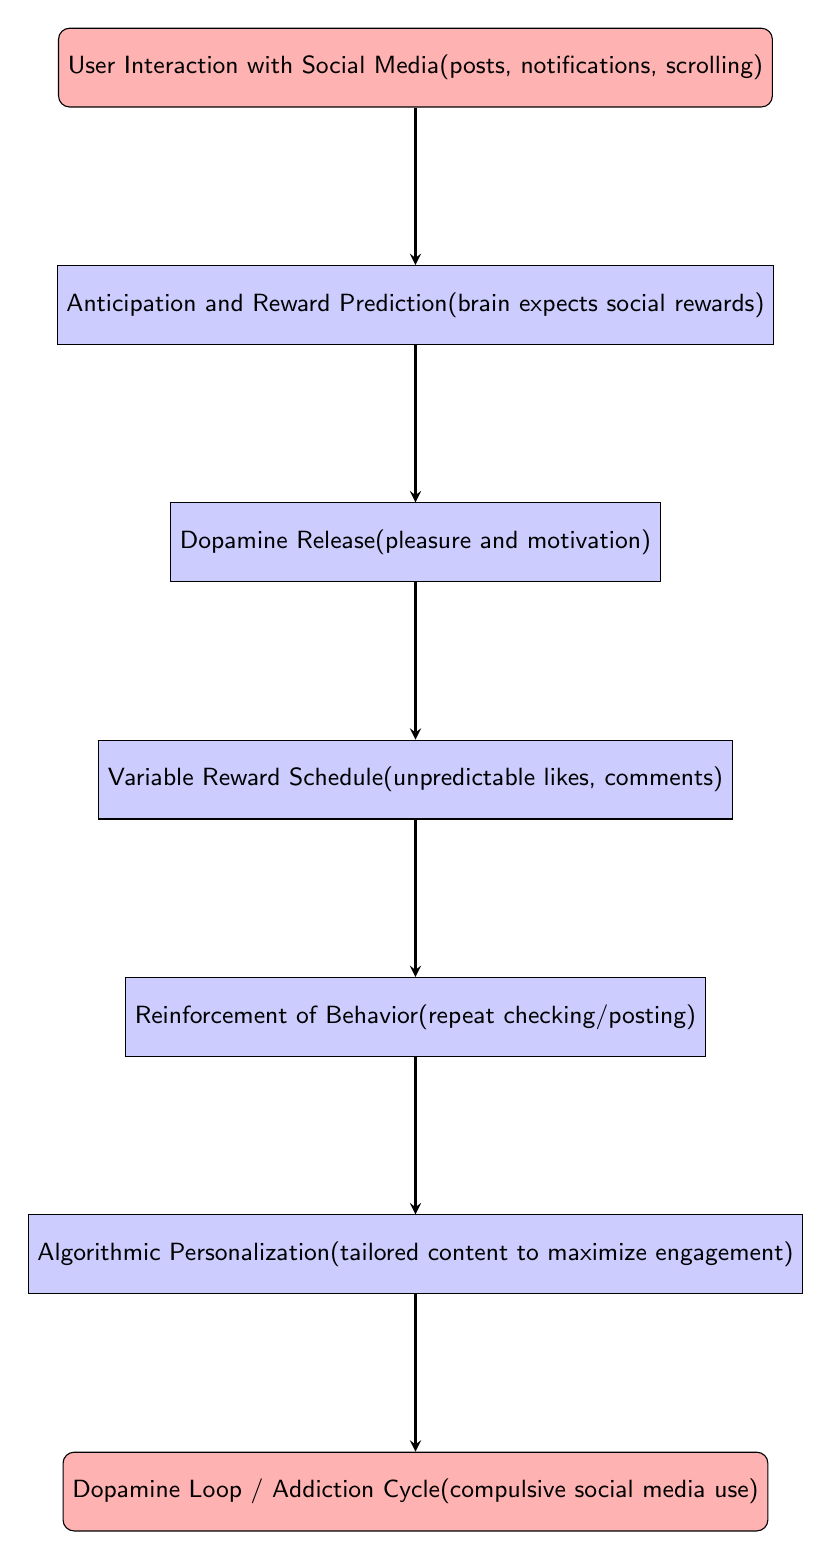
\begin{tikzpicture}[node distance=2cm, every node/.style={font=\small}]

\tikzstyle{startstop} = [rectangle, rounded corners, minimum width=3cm, minimum height=1cm, text centered, draw=black, fill=red!30]
\tikzstyle{process} = [rectangle, minimum width=3.5cm, minimum height=1cm, text centered, draw=black, fill=blue!20]
\tikzstyle{arrow} = [thick,->,>=stealth]

% Nodes
\node (interaction) [startstop] {User Interaction with Social Media \\ (posts, notifications, scrolling)};
\node (anticipation) [process, below=of interaction] {Anticipation and Reward Prediction \\ (brain expects social rewards)};
\node (dopamine) [process, below=of anticipation] {Dopamine Release \\ (pleasure and motivation)};
\node (variable) [process, below=of dopamine] {Variable Reward Schedule \\ (unpredictable likes, comments)};
\node (reinforcement) [process, below=of variable] {Reinforcement of Behavior \\ (repeat checking/posting)};
\node (algorithm) [process, below=of reinforcement] {Algorithmic Personalization \\ (tailored content to maximize engagement)};
\node (loop) [startstop, below=of algorithm] {Dopamine Loop / Addiction Cycle \\ (compulsive social media use)};

% Arrows
\draw [arrow] (interaction) -- (anticipation);
\draw [arrow] (anticipation) -- (dopamine);
\draw [arrow] (dopamine) -- (variable);
\draw [arrow] (variable) -- (reinforcement);
\draw [arrow] (reinforcement) -- (algorithm);
\draw [arrow] (algorithm) -- (loop);

\end{tikzpicture}

Have we ever thought about why there’s no end to newsfeed scrolling or reel watching? The continuous notifications or pull-to-refresh features make us spend a long time on social media. Sometimes, we pick up our phone just because of a notification sound from social media, only to end up wasting an hour for no real reason. These platforms are designed to trigger dopamine release, creating a rewarding cycle that keeps users coming back for more. The brain’s reward system responds to likes, comments, and shares, releasing small bursts of dopamine with each interaction. This neurochemical response reinforces the behavior, making social media use habit-forming and potentially addictive. These features also cause FOMO (fear of missing out), which leads teens to get addicted to social media influence and reach.

One of the most concerning aspects is the algorithm that serves us our preferred content. Ever wondered how social media knows what your favorite content is and which contents tend to keep you long time on screen? You might discuss the "Final Destination" movie with friends, and the next day your Instagram reels are filled with related content. Or you text a friend about needing an ESP32 microcontroller for a project, and suddenly you see ads for it everywhere.

How do they know what you need? The answer is simple: we give permissions like location, voice, and camera to the social media app. Using all those permissions, they analyze our personal data along with our posts or interaction data through artificial intelligence. Then they display specific content or items. Once I stared at a person’s story for a few seconds, and then Facebook started to show that person’s posts and stories at the top of my feed. That’s how their algorithms function—to keep us on their apps for as long as possible.

\section*{Breaking the Habit}

Breaking the cycle of social media addiction begins with awareness. Setting boundaries, such as limiting screen time, turning off non-essential notifications, and creating tech-free zones, can help reduce compulsive use. Practicing mindfulness, pausing to ask why you are reaching for your phone can help you regain control. Engaging in activities that naturally boost dopamine, such as exercise, creative hobbies, or spending time with friends and family can provide healthier sources of reward. Understanding how social media is designed to capture your attention empowers you to make more intentional choices about your digital habits. With conscious effort, it is possible to reclaim your time and attention from the grip of digital dopamine triggers.

\section*{References}

\begin{enumerate}
    \item Volkow, N. D., \& Morales, M. (2015). The Brain on Drugs: From Reward to Addiction. \textit{Neuron, 87}(4), 638–654. \href{https://www.cell.com/neuron/pdf/S0896-6273(15)00133-6.pdf}{PDF Link}
    \item Webmedy. Dopamine and Decision Making. \href{https://webmedy.com/blog/dopamine-decision-making/}{https://webmedy.com/blog/dopamine-decision-making/}
    \item OurMental.Health. Hooked on Dopamine. \href{https://www.ourmental.health/screen-time-sanity/hooked-on-dopamine-how-social-media-hijacks-your-brain}{https://www.ourmental.health/...}
    \item Neurolaunch. Social Media and Dopamine. \href{https://neurolaunch.com/social-media-dopamine/}{https://neurolaunch.com/social-media-dopamine/}
    \item Glass Almanac. How Dopamine Influences Behavior and Decision-Making According to Science. \href{https://glassalmanac.com/how-dopamine-influences-behavior-and-decision-making-according-to-science/}{https://glassalmanac.com/...}
    \item Healthline. Dopamine Addiction. \href{https://www.healthline.com/health/dopamine-addiction}{https://www.healthline.com/health/dopamine-addiction}
    \item Verywell Mind. Can You Get Addicted to Dopamine? \href{https://www.verywellmind.com/can-you-get-addicted-to-dopamine-5207433}{https://www.verywellmind.com/...}
\end{enumerate} 
% PASTE ARTICLE 7 CONTENT HERE

% ====================
% CONTRIBUTORS PAGE
% ====================
\clearpage
\section*{Contributors}
\addcontentsline{toc}{section}{Contributors}
\vspace*{0.2cm}  % Reduce top space

% Compact contributor entries without images
\contributor{Muhaimin Kamran}{366}{20240659148}{}
\contributor{Maliha Laheen}{322}{20240659104}{}
\contributor{Ferdous Ara Fahima}{323}{20240659105}{}
\contributor{Tamjeed Rahman Udoy}{373}{20240659155}{}
\contributor{Sultana Akter}{325}{20240659107}{}
\contributor{Md. Kaif Ibn Zaman}{358}{20240659140}{}
\contributor{Md. Asif Khan}{348}{20240659130}{}


\begin{figure}[ht]
  \hspace{2.0cm}
  
\includegraphics[width=0.8\textwidth]{group_photo.jpg}
\end{figure}

% ====================
% BACK PAGE
% ====================
\clearpage
\thispagestyle{empty}
\begin{center}
\begin{minipage}{\textwidth}
\centering
\vspace*{\fill}
\vspace{8.5cm}

{\Large\itshape\color{primary}``Great stories begin with curious minds and courageous voices.''}

\vspace{0.8em} % Tighter spacing
{\large\bfseries\color{dark}— NeuroNumb}

\vspace{1.5cm} % Reduced space
\tikz{\draw[accent, line width=0.5pt] (0,0) -- (5cm,0);}

\vspace{0.8em} % Tighter spacing
{\large\scshape\color{dark}The Aevum}

\vspace{0.3em} % Tighter spacing
{\small\color{gray}Volume 1 • June 2025}

\vspace{0.3em} % Tighter spacing
% {\footnotesize\color{gray}www.teammagazine.com • contact@teammagazine.com}

\vspace*{\fill}
\end{minipage}
\end{center}

\end{document}
